%!TEX root = ../deco_star.tex

%-------------------------------------------------------------------------
\section{Design Features}
\label{sec:design}

For the analysis of the state of the art we sort the work into design areas, hence the visual features they enable. Within those design areas we are then discussing the control mechanisms.

In regard to design features, on the one hand, creative pattern generation includes repetitive and ordered structures that are often considered as \textit{textures}, thus demanding automatic and procedural creation. On the other hand, creative pattern generation might also include a global layout, adapting to the space they are filling. Furthermore, this type of patterns might include visual hierarchies and highlights that are singularly placed with creative intent. 
% With that creative pattern generation is an interesting testing ground for addressing the delicate balance between giving artists as much control as is needed without burdening them with unwanted details.

Specifically, we categorize the analysis of the state of the art in \Cref{sec:analysis} on the following potential design features for creative pattern generation:

% TODO: Add graphic for each category?

\begin{itemize}
    \item Distribution and Repetition
    \item Frames and Hierarchies
    \item Curves, Lines and Brushing
    \item Connections, Branches and Directionality
    \item Single Accents
\end{itemize}

For these features, ornamentation constitutes an illustrative example of a creative pattern generation task and includes all of the above visual characteristics. Even though this survey investigates a more general design space, in the following we are briefly summarizing the specific design goal of ornamentation for a better understanding overall. 

\subsection{Ornamentation}
\label{subsubsec:ornamentation}

% The Oxford English Dictionary~\cite{oed_2017} defines ornaments as nonessential accessories intended to adorn.
There is no functionality to an ornament other than to beautify a manufactured article without changing its shape or character~\cite{ward_1896_tpo}.
% The term ornament can be found in a large variety of contexts, such as in architecture, music or poetry, but this work only refers to two-dimensional visual ornaments. 
% While ornaments may carry symbolic meanings in the arranged elements \cite{wornum_1896_aof}, this work does not include semantics but focuses on visual qualities. 
Different cultures and times resulted in various ornamental styles, with great differences in the details as \Cref{fig:historic_examples} shows. Nevertheless common underlying design principles for ornamentation can be identified.

\begin{figure}
    % \centering
       \includegraphics[width=1.0\columnwidth]{figures/historic_examples/examples.jpg}
       \bb{I replaced it with JPG for faster compilation. Replace with PNG for the submission.}
        \caption[Historic pattern examples]{\label{fig:historic_examples} Historic examples for creative pattern designs and ornamentation. Places of origin from left to right, top to middle row:  France, China, USA, UK, Poland, Egypt, UK (cutout of a tiled pattern). Bottom row: recent commercial examples. This figure is adapted from~\cite{gieseke_2017_ooo}, image sources: [1-10].}
\end{figure}

Ornamentation can be understood as an accurately defined type of decor that follows a structural logic~\cite{ward_1896_tpo, moughtin_1999_udo, arbruzzo_2006_dec}. 
% But the transition between formal ornamentation and informal decoration is smooth, with various common aspects~\cite{moughtin_1999_udo}. 
In addition to its aesthetic appeal, an ornament is perceptually distinguished by a sense of order and by its alignment to the space it fills (as discussed by \cite{wong_1998_cgf,gieseke_2017_ooo} and originally stated by \citeauthor*{ward_1896_tpo}~\cite{ward_1896_tpo, dresser_1875_pdd, arbruzzo_2006_dec}). 


%  \citeauthor*{arbruzzo_2006_dec}~\cite{arbruzzo_2006_dec} elaborate on ornamentation as follows:

% \begin{quote}
% \textit{[An] ornament is inextricable linked to scale and proportion, to form and order. In this context, the modus operandi of ornamentation is always to reinforce an existing order: to conform to its partner in the ornament-object relationship, for ornament always has a partner in that which is ornamented.}
% \end{quote}

An underlying perception of order in an ornament is established by even repetition and a balanced distribution of elements, with an intentionally designed and artificial quality~\cite{ward_1896_tpo}. Balance can be achieved with a careful composition of elements, and such balance is built on symmetrical arrangements in most ornaments \cite{gieseke_2017_ooo}. Compositions are not limited to the repetition of the same element, but different visual qualities such as size or saturation can create various relationships. 

% Visual characteristics attract the eye differently and the \textit{visual weight} of a feature can be used as a measure for the degree of attraction. For example, large, dark and highly saturated colored elements have a greater visual weight than small, light and desaturated ones. These visual weights can be used to create visual correlations (for example, based on Gestalt psychology - a topic too wide for a discussion here) and can counterbalance each other. A larger and lighter colored element might have the same visual weight as a smaller, darker colored one. Hence, varied elements with different visual properties can be combined and still make a balanced whole.

Hierarchical compositions further increase a sense of order but are also used for creating contrasts (e.g., foreground vs. background) and accentuating structures (e.g., framing). These structures are often used to elaborate and accentuate the form of the space they fill, building an ornament-object relationship \cite{arbruzzo_2006_dec}. The following differentiation of an ornamental decoration gives an intuitive understanding of this aspect~\cite{arbruzzo_2006_dec}: Wallpaper can be trimmed for different rooms, but the design is not reproportioned or altered. An ornament, however, is fitted to and references the logic of the space it is designed for. Without adjustment, it cannot be transferred to a different space.

Contrasts and accents are crucial for the visual appeal of an ornament~\cite{wong_1998_cgf,ward_1896_tpo, moughtin_1999_udo}. Single, visually dominant elements and structures might not follow the underlying order of the ornament at all, breaking an otherwise too homogeneous appearance - again distinguishing ornamentation from wallpaper.

\Cref{fig:ornamentation_principles} gives an example of how the described design principles are combine seamlessly into a coherent design.

% As \citeauthor*{gieseke_2017_ooo}~\cite{gieseke_2017_ooo} state, it takes artistic expertise to balance the contrast between carefully 

As we have stated in previous work~\cite{gieseke_2017_ooo}, it takes artistic expertise to balance the contrast between carefully chosen visual accents and to create a sense of order by applying compositional rules and by complementing the space. However, it is exactly this combination of qualities - rule-based composition and repetition on the one hand and the placement of visual accents and the breaking free from order on the other.
% - that make creative pattern generation an interesting but highly challenging field of algorithmic research in the context of computer graphics.


\begin{figure}
    % \centering
       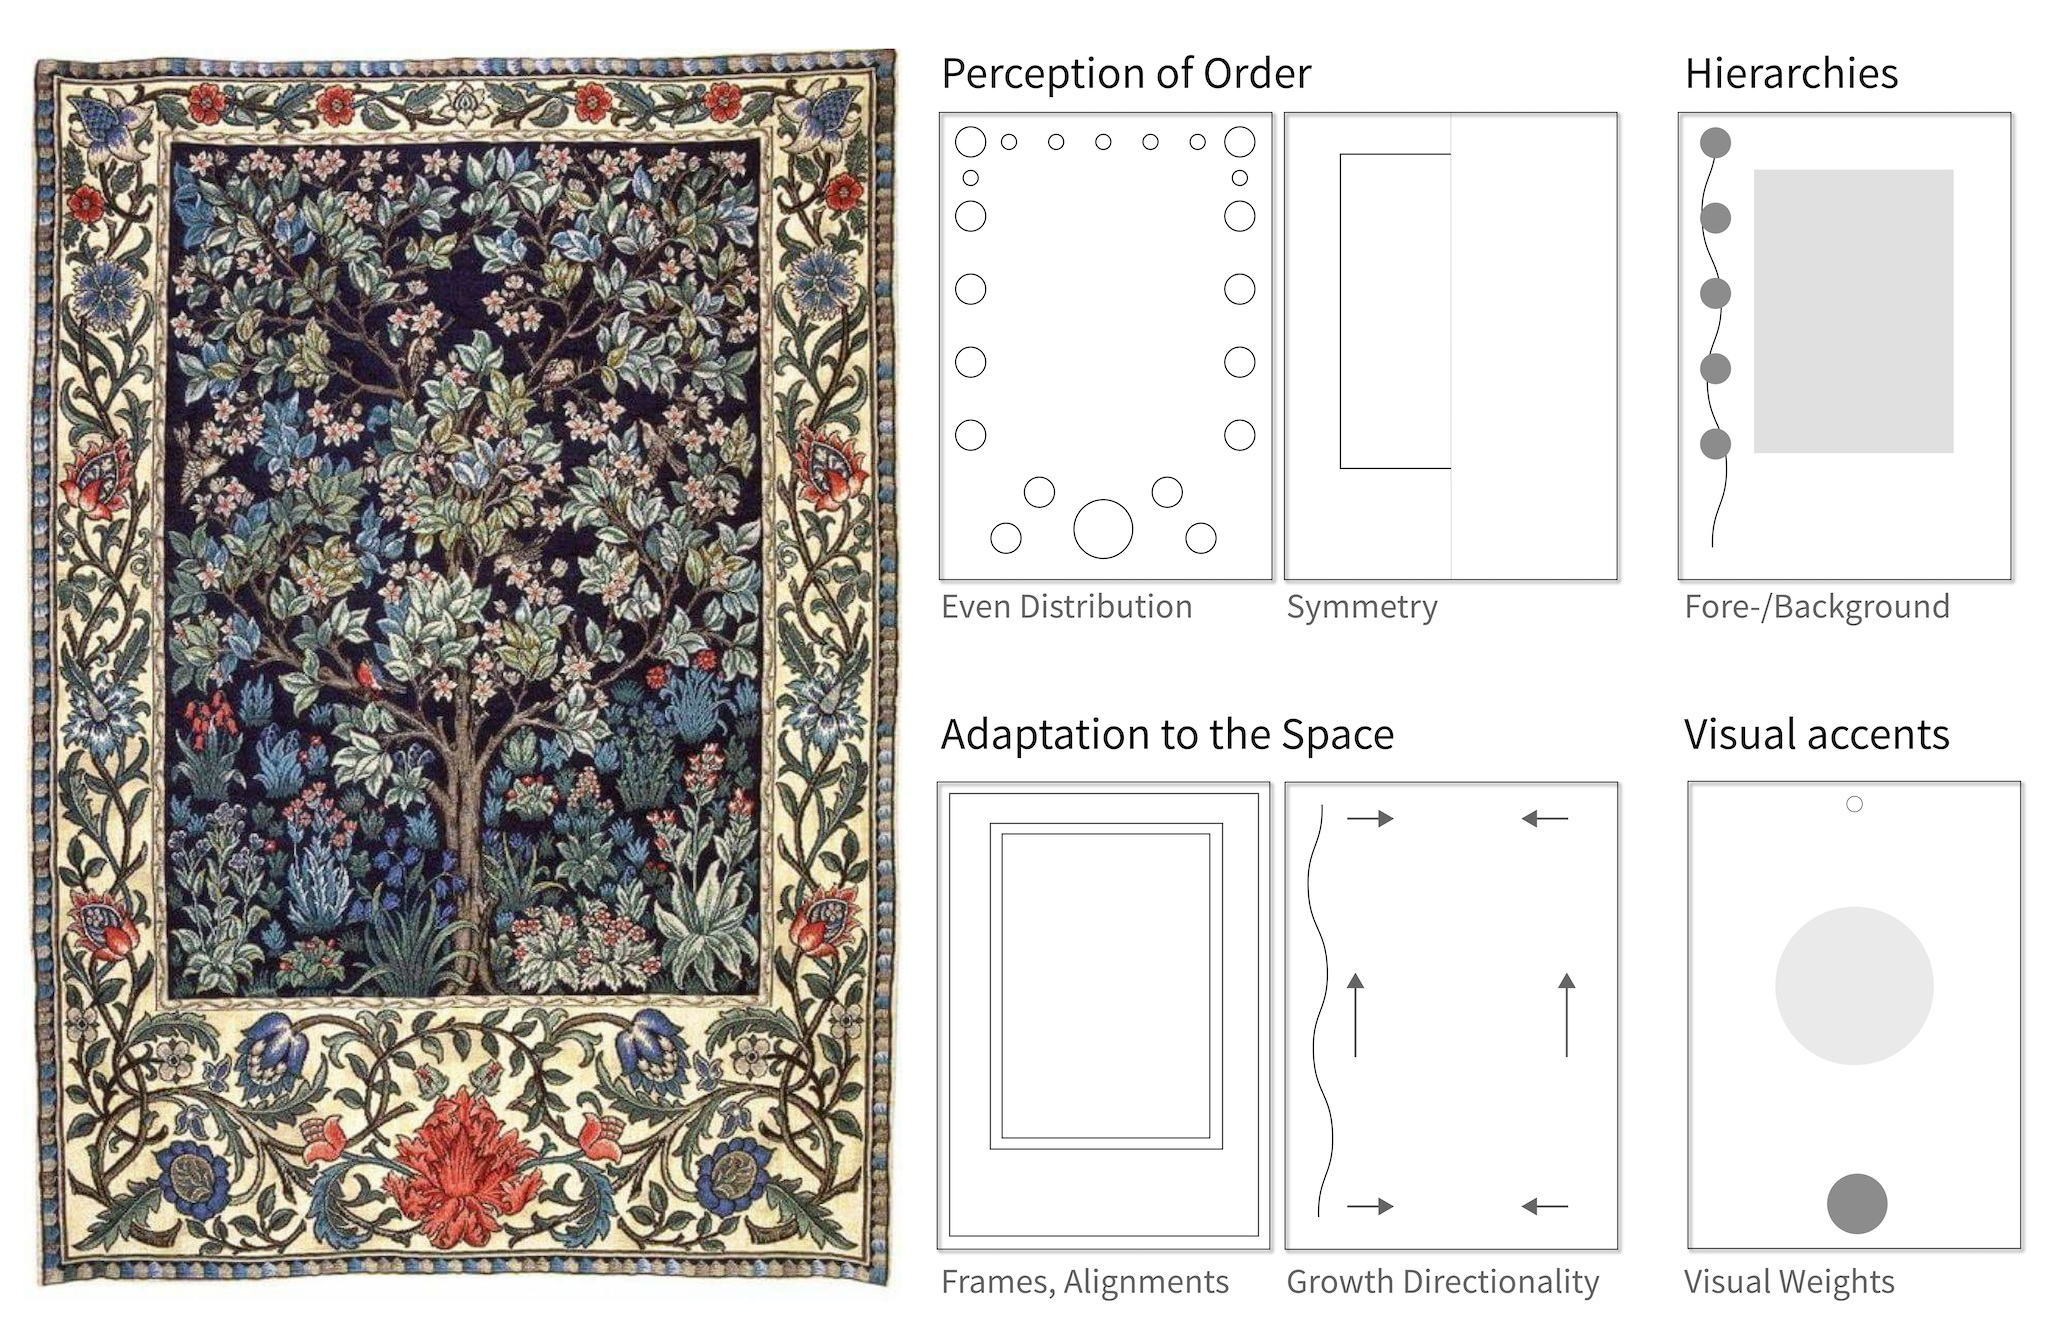
\includegraphics[width=1\columnwidth]{figures/ornament/ornament_principles.jpg}
       \bb{I replaced it with JPG for faster compilation. Replace with PNG for the submission.}        \caption[Ornamentation principles]{\label{fig:ornamentation_principles} Exemplary dissection of visual characteristics fulfilling ornamental principles. Single features often support several principles, as, for example, the frames and borders create a hierarchical composition, an adaption to the space the ornament fills and visual contrasts. Image source left image: [11]}
\end{figure}

% \subsection{Summary}
% \label{subsec:design_summary}

% Creative pattern generation differentiates itself from homogeneous pattern creation by including aspects such as distribution and repetition, curves, lines and sketches, frames and hierarchies, connections, branches and directionality, and single accents. Creative pattern generation exemplifies the common challenge of enabling control for tasks for which humans are indispensable in combination with the automation of tedious manufacturing and the computation of structuring rules. With that it is a representative design goal to aspire to for a general investigation of creative control mechanisms.
